\documentclass{article} % For LaTeX2e
\usepackage[backend=bibtex]{biblatex}
\addbibresource{bibliography.bib}
\usepackage{graphicx}
\graphicspath{{figures/}}
\usepackage{nips15submit_e,times}
\usepackage{hyperref}
\usepackage{url}
\usepackage{amsmath}
\usepackage{tipa}
\usepackage{multicol}
\usepackage{multirow}
\usepackage[linesnumberedhidden,ruled,noend]{algorithm2e}
\usepackage{listings}
\usepackage{color}

\definecolor{dkgreen}{rgb}{0,0.6,0}
\definecolor{gray}{rgb}{0.5,0.5,0.5}
\definecolor{mauve}{rgb}{0.58,0,0.82}

\lstset{frame=tb,
  language=Python,
  aboveskip=3mm,
  belowskip=3mm,
  showstringspaces=false,
  columns=flexible,
  basicstyle={\small\ttfamily},
  numbers=none,
  numberstyle=\tiny\color{gray},
  keywordstyle=\color{blue},
  commentstyle=\color{dkgreen},
  stringstyle=\color{mauve},
  breaklines=true,
  breakatwhitespace=true,
  tabsize=3
}

\makeatletter
\def\BState{\State\hskip-\ALG@thistlm}
\makeatother
%\documentstyle[nips14submit_09,times,art10]{article} % For LaTeX 2.09

\title{COMPGW02: Web Economics\\Assignment 1 - Part A}

\author{
Sergiu Tripon\\
Department of Computer Science\\
University College London\\
Gower Street, London, WC1E\\
\texttt{sergiu.tripon.15@ucl.ac.uk}\\
}

% The \author macro works with any number of authors. There are two commands
% used to separate the names and addresses of multiple authors: \And and \AND.
%
% Using \And between authors leaves it to \LaTeX{} to determine where to break
% the lines. Using \AND forces a linebreak at that point. So, if \LaTeX{}
% puts 3 of 4 authors names on the first line, and the last on the second
% line, try using \AND instead of \And before the third author name.

\newcommand{\fix}{\marginpar{FIX}}
\newcommand{\new}{\marginpar{NEW}}

\nipsfinalcopy % Uncomment for camera-ready version

\begin{document}

\maketitle

\section{REAL-TIME BIDDING \cite{easley2010networks}}

\section*{Question 1}

In a second price auction, with a single and indivisible item, the dominant strategy is truthful bidding. That is, each bidder will bid their true value of the item. In this context, we know the advertiser's true value for each user click on the ad and we also know the click-through rate on the ad. Therefore, her truthful bidding \textit{b\textsubscript{i}} will be:

\[ b_i = r_i \]

where \textit{b\textsubscript{i}} is advertiser \textit{i}'s truthful bidding on the bid request and \textit{r\textsubscript{i}} is her true value for each user click on her ad.

Let's take advertisers \textit{p} and \textit{i} with true values \textit{r\textsubscript{p}} and \textit{r\textsubscript{i}}, respectively. If both \textit{p} and \textit{i} use the truth telling bidding strategy, in a second price ad auction, they will always bid their true value of the item, and therefore, if their value of the item is the same, they will bid the same price for each auction:

\[ b_p = r_p \]
\[ b_i = r_i \]

In order to prove this we need to verify that if \textit{p} bids \textit{b\textsubscript{p} = r\textsubscript{p}}, there is no other strategy that would improve advertiser \textit{p}'s payoff, regardless of the bidding strategy employed by any other advertiser. Below, we will verify two hypothetical scenarios where \textit{p} increases or decreases their bid.

In both hypothetical scenarios, it is important to consider that the value that \textit{p} bids only has an impact on whether \textit{p} wins or loses the auction. However, it does not have any impact on what \textit{p} will pay in the event where \textit{p} wins, as the amount to be paid is determined by the other bids, more specifically by the largest of the other bids.

Firstly, let's assume that instead of advertiser \textit{p} bidding \textit{r\textsubscript{p}}, they actually bid \textit{b\textsubscript{p} \textgreater r\textsubscript{p}}. This only has an impact on \textit{p}'s payoff, if \textit{p} would lose with bid \textit{b\textsubscript{p} = r\textsubscript{p}} but \textit{p} would win with bid \textit{b\textsubscript{p} \textgreater r\textsubscript{p}}. For this to happen, the other highest bid \textit{p\textsubscript{k}} must be between \textit{b\textsubscript{p} = r\textsubscript{p}} and \textit{b\textsubscript{p} \textgreater r\textsubscript{p}}. In this case, \textit{p}'s payoff would be maximum $r_p - b_p \le 0$, which does not increase \textit{p}'s payoff.

Secondly, let's assume that instead of advertiser \textit{p} bidding \textit{r\textsubscript{p}}, they actually bid \textit{b\textsubscript{p} \textless r\textsubscript{p}}. This only has an impact on \textit{p}'s payoff, if \textit{p} would win with bid \textit{b\textsubscript{p} = r\textsubscript{p}} but \textit{p} would lose with bid \textit{b\textsubscript{p} \textless r\textsubscript{p}}. For this to happen, the other highest bid \textit{p\textsubscript{k}} must be between \textit{b\textsubscript{p} = r\textsubscript{p}} and \textit{b\textsubscript{p} \textless r\textsubscript{p}}. In this case, \textit{p}'s payoff would be 0 because \textit{p} loses, which does not increase \textit{p}'s payoff.

Figure \ref{fig:web_economics_1} provides a visual representation of this proof.

\begin{figure}[ht]
\centering
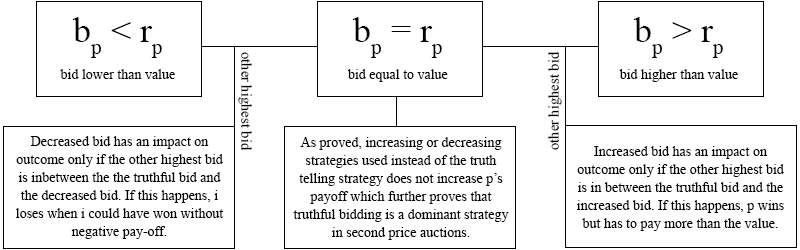
\includegraphics[width=1\textwidth]{web_economics_1}
\caption{Proof of why truthful bidding is a dominant strategy in second price auctions.}
\label{fig:web_economics_1}
\end{figure}

\section*{Question 2}

The right choice of changing her truth-telling bid price in order to maximise the ad click number is to keep the bid price level.

In \textit{Question 1}, it has been proved that any deviation from the advertiser's true value-based bid \textit{b\textsubscript{i}} = \textit{r\textsubscript{i}} would not improve her payoff and is not optimal. On the other hand, the advertiser bidding their true value is optimal. This makes truthful bidding a dominant strategy in second price auctions, with a single and indivisible item.

It is not optimal for advertiser \textit{i} to bid more than her true value, because it will only help her to win the slot if the second highest bidder's bid is at least equal to her true value. In this scenario, advertiser \textit{i} will not gain anything, but may lose something.

It is not optimal for advertiser \textit{i} to bid less than her true value, because her bid does not have an impact on the price she has to pay if she wins the slot. In this scenario, advertiser \textit{i}'s lower bid may make her lose the slot even thought it would've been advantageous for her to win it as the price is lower than her true value.

\section{SPONSORED SEARCH AUCTION \cite{easley2010networks} \cite{easley2010networks1}}

The contents of my \textit{Auction.py} file can be found, below.

\begin{lstlisting}
# Auction.py

#!/usr/bin/python
import Bid, Slot

class Auction:
	'This class represents an auction of multiple ad slots to multiple advertisers'
	query = ""
	bids = []

	def __init__(self, term, bids1=[]):
		self.query = term

		for b in bids1:
			j=0
			print(len(self.bids))
			while j<len(self.bids) and float(b.value) <float(self.bids[j].value):
				j+=1
			self.bids.insert(j,b)

	'''
	This method accepts a Vector of slots and fills it with the results
	of a VCG auction. The competition for those slots is specified in the bids Vector.
	@param slots a Vector of Slots, which (on entry) specifies only the clickThruRates
	and (on exit) also specifies the name of the bidder who won that slot,
	the price said bidder must pay,
	and the expected profit for the bidder.  
	'''

	def executeVCG(self,slots):
		# TODO: implement this method
		# print ("executeVCG: To be implemented")

		price = 0.0
		lowClickThruRate = 0.0

		# for loop as many times as number of slots, descending >> if 4 slots, it will loop: 3, 2, 1, 0
		for bid in range(len(slots)-1, -1, -1):
			# if bid no. is smaller than number of bids, continue
			if bid < len(self.bids):
				# if current bid no. + 1 is smaller than number of bids, do calculations
				if bid+1 < len(self.bids):
					# calculate price: bid amount * (current slot's clickThruRate - lowClickThruRate)
					price += self.bids[bid+1].value * (slots[bid].clickThruRate - lowClickThruRate)
				# assign current bidder's price
				slots[bid].price = price
				# assign current bidder's name
				slots[bid].bidder = self.bids[bid].name
				# calculate and assign current bidder's profit: (bid amount * clickThruRate) - price
				slots[bid].profit = (self.bids[bid].value * slots[bid].clickThruRate) - slots[bid].price
			# if bid no. is larger than number of bids, assign zero values
			elif bid > len(self.bids):
				# assign zero value to current bidder's price
				slots[bid].price = 0
				# assign zero value to current bidder's name
				slots[bid].bidder = 0
				# assign zero value to current bidder's profit
				slots[bid].profit = 0
			# assign current slot's clickThruRate to lowClickThruRate
			lowClickThruRate = slots[bid].clickThruRate
\end{lstlisting}

\printbibliography
\end{document}